
\section{Evaluation}
\label{sec:evaluation}

We evaluated four aspects of \ourtool's effectiveness,
answering the following research questions:

\begin{itemize}
\item What is the success ratio of \ourtool in synthesizing
SQL queries? (Section~\ref{sec:ratio}).
%Is the supported SQL subset expressive enough to describe a variety of queries?
\item How long does it take for \ourtool to
synthesize a SQL query (Section~\ref{sec:performance}).
\item How much human effort is needed to write sufficient
input-output examples for SQL synthesis (Section~\ref{sec:human}).
\item How does \ourtool's effectiveness compare to
existing SQL query inference techniques (Section~\ref{sec:comparison}).
\end{itemize}






\subsection{Benchmarks}

%We collected benchmarks from two sources, and show them 
%in Figure~\ref{tab:results}.

Our benchmarks are shown in Figure~\ref{tab:results}.


\begin{itemize}
\item We used \allex SQL query related exercises
from a classic database textbook~\cite{cowbook}.
These exercises are from Chapter 5, which systematically
introduces the SQL language. We chose textbook exercises because they
are designed to
cover a wide range of SQL features. Some exercises
are even designed on purpose to cover some less realistic,
corner cases in using SQL. 
%all exercises are about
%writing a SQL query that retrieve data from a database.
We used \textit{all} exercises that can be answered using the standard
SQL language features without any vendor-specific
features or user-defined numeric functions.
As shown in Figure~\ref{tab:results},
most textbook exercises involve at least 3 tables. It was unintuitive
for us to write the correct query by simply looking at the problem
description.

\item We searched SQL query related questions raised by real-world
database users from 3 popular online forums~\cite{stackoverflow,
tutorialized, dbjournal}.
We focused on questions about how to use standard SQL features.
We excluded questions that were vaguely described or obviously
wrong, and discarded questions that had been proved
to be unsolvable by using SQL (e.g., computing a
transitive closure).
We collected \pnum non-trivial forum questions related to writing a SQL query
(available at:~\cite{forumq}), among which
two questions even did not receive any reply.
Writing a good forum post is often harder than asking
a SQL expert (since the post has to clearly 
describe the problem), and these end-users had already tried but
failed to find the correct SQL query before they wrote the post.
\end{itemize}



\subsection{Evaluation Procedure}

We used \ourtool to solve each textbook exercise and forum
question. If an exercise or problem
was associated with example input and output,
we directly applied \ourtool on those examples.
Otherwise, we manually wrote some example input and output.
To reduce the bias in writing
examples, all examples are written by a graduate
student (whose research field is not database-related) from University of Washington rather than
\ourtool's developers.

We checked \ourtool's correctness by comparing its
output with the expected SQL queries.
For textbook exercises, we compared \ourtool's output with
their correct answers; for forum questions, we first
checked \ourtool's output with the confirmed answer
in the same post, if there is any. Otherwise, we
manually wrote the correct SQL query and then
compared it with \ourtool's output.
%determined
%whether \ourtool can produce it.
%the output query can fulfill
%the query task or not.

For some textbook exercises and forum questions,
\ourtool inferred a SQL query that satisfied the input-output
examples, but did not behave as expected.
We manually found an input on which the
SQL query mis-behaved and re-applied \ourtool to the new input. We
repeated this process and recorded the total number of
interactions.
% before \ourtool output a correct SQL query.


All experiments were run on a 2.67GHz Intel Core PC
with 4GB physical memory, running Windows 7.



\begin{figure*}[t]
\setlength{\tabcolsep}{.24\tabcolsep}
\begin{tabular}{|c|l|c||c|c|c|c|c||l|}
\hline
\multicolumn{3}{|c||}{Benchmarks} & \multicolumn{5}{|c||}{\ourtool} & Query by\\
\cline{1-8}
 ID & Source & \#Input Tables & Example Size & Rank & Time Cost (s) & Cost in Writing Examples (m) & \#Iterations & Output~\cite{Tran:2009}\\
 \hline
 \hline
 1 &Textbook Ex 5.1.1 & 4 &  & & & & & \\
 2 &Textbook Ex 5.1.2 & 4&  & & & & & \\
 3 &Textbook Ex 5.1.3 & 4&  & & & & & \\
 4 &Textbook Ex 5.1.4 & 4&  & & & & & \\
 5 &Textbook Ex 5.1.5 & 4&  & & & & & \\
 6 &Textbook Ex 5.1.6 & 4&  & & & & & \\
 7 &Textbook Ex 5.1.7 & 4&  & & & & & \\
 8 &Textbook Ex 5.1.8 & 4&  & & & & & \\
 9 &Textbook Ex 5.1.9 & 4&  & & & & & \\
 10 &Textbook Ex 5.1.10 & 4&  & & & & & \\
 11 &Textbook Ex 5.1.11 & 4&  & & & & & \\
 12 &Textbook Ex 5.1.12 & 4&  & & & & & \\
 13 &Textbook Ex 5.2.1 & 3 &  & & & & & \\
 14 &Textbook Ex 5.2.2 & 3&  & & & & & \\
 15 &Textbook Ex 5.2.3 & 3&  & & & & & \\
 16 &Textbook Ex 5.2.4 & 3&  & & & & & \\
 17 &Textbook Ex 5.2.5 & 3&  & & & & & \\
 18 &Textbook Ex 5.2.6 & 3&  & & & & & \\
 19 &Textbook Ex 5.2.7 & 3&  & & & & & \\
 20 &Textbook Ex 5.2.8 & 3&  & & & & & \\
 21 &Textbook Ex 5.2.9 & 3&  & & & & & \\
 22 &Textbook Ex 5.2.10 & 3&  & & & & & \\
 23 &Textbook Ex 5.2.11 & 3&  & & & & & \\
 24 &Forum Question 1 & &  & & & & & \\
 25 &Forum Question 2 & &  & & & & & \\
 26 &Forum Question 3 & &  & & & & & \\
 27 &Forum Question 4 & &  & & & & & \\
 28 &Forum Question 5 & &  & & & & & \\
\hline
\end{tabular}
\Caption{{\label{tab:results} Experimental results of SQL query synthesis.
Column ``Benchmarks'' describes the characteristics of our benchmarks. Sub-column ``\#Input Tables''
shows the number of input tables in each benchmark. Column ``\ourtool'' shows
\ourtool's results. Sub-column ``Example Size''
shows the number of tuples (i.e., rows) in all example input and output tables.
Sub-column ``Rank'' shows the absolute
rank of the correct SQL query in \ourtool's output.
``\textbf{X}'' means \ourtool fails to produce a correct answer.
Sub-column ``Cost in Writing
Examples (m)'' shows the total time cost of writing sufficient
examples in minutes. Sub-column ``\#Iterations'' shows the number of
interactive rounds in using \ourtool to obtain the correct query.
Column ``Query by Output'' shows the results of using an existing
technique, called
\textit{Query by Output} (QBO)~\cite{Tran:2009}. In this column,
``\textbf{Y}''  means QBO produces the correct SQL query, and ``\textbf{N}''
means QBO fails to produce the correct query.
Since QBO was implemented as a special case in \ourtool; its
time cost is similar to \ourtool and is omitted for brevity.
}}
\end{figure*}



\subsection{Results}

Figure~\ref{tab:results} summarizes our experimental results.

\subsubsection{Success Ratio}
\label{sec:ratio}


\ourtool synthesized correct SQL queries for \solexnum  out of
\exnum the textbook exercises, and 
all \pnum forum questions.
\ourtool failed to solve XXX textbook exercises, for
two reasons. XXX exercises 
%per exercise (or problem).
\todo{why the technique can work, why some problem
can not be solved}

We also observed that our ranking strategy (Section~\ref{sec:ranking})
was quite effective: for most benchmarks, it ranked the correct
SQL query as one of top XXX suggestions.

%

\begin{figure*}[t]
  \centering
  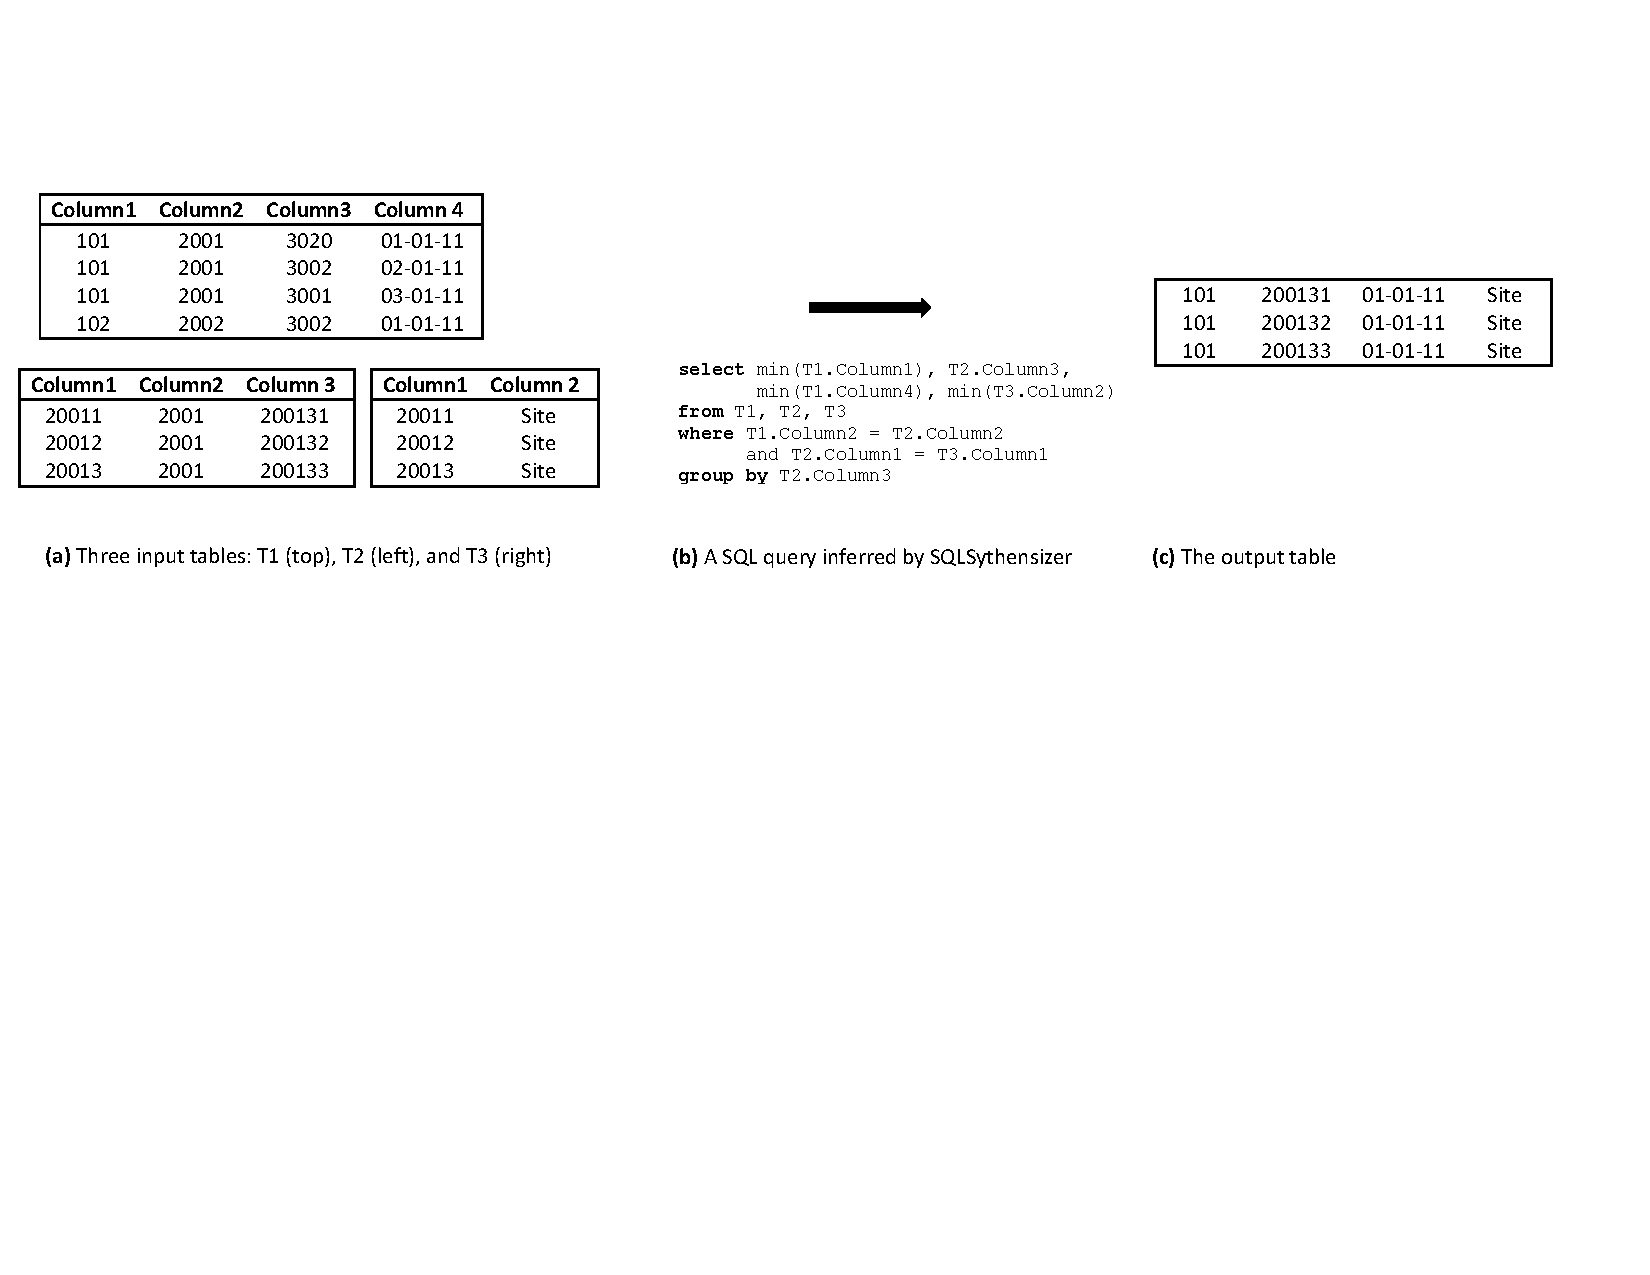
\includegraphics[scale=0.70]{example2}
  \vspace*{-1.0ex}\caption {{\label{fig:example2} Input-output
  examples ((a) and (c)) taken from an online SQL help forum
  thread. \ourtool automatically sythensizes 6 SQL queries that
  can produce the output table from the three input tables.
  (b) shows the highest ranked SQL query.
}}
\end{figure*}

We use a real SQL question from
an online forum\footnote{\url{http://forums.tutorialized.com/sql-basics-113/join-problem-147856.html}} to illustrate
\ourtool's effectiveness.
The question was started by a novice user, who needed help to write a
SQL query to get result from three input tables. In this question, the
novice user described his required query in a few paragraphs of
English, but also include several small, representative input-output
examples as shown in Figure~\ref{fig:example2}, to better express
his intention. 
This question receives no replies as of April 2013 and we speculated that
writing a SQL query to join three tables to produce certain output results
is non-trivial.

We ran \ourtool on the input-output examples
in Figure~\ref{fig:example2}. The tool produced 6 valid answers
in less than 1 minutes, all of which satisfy the given examples. The
highest ranked SQL query is shown in Figure~\ref{fig:example2},
which is quite unintuitive to write. The SQL query in
Figure~\ref{fig:example2}
first joins three input tables
on columns \CodeIn{T1.Column2}, \CodeIn{T2.Column2},
\CodeIn{T2.Column1}, and \CodeIn{T3.Column1} using some
selected columns, and then aggregates the results based on
column \CodeIn{Table2.Column3}'s value. Finally, it
returns the minimal values of columns \CodeIn{T1.Column1}, \CodeIn{T1.Column4}, and \CodeIn{T3.Column2}
from each aggregated group as the results.




\subsubsection{Performance}
\label{sec:performance}

%We measured \ourtool's performance by recording the
%time cost in producing a ranked list of SQL queries.
On average,
including benchmarks that \ourtool failed to produce
a correct answer,
\ourtool took less than \avgtime minutes in total to
produce the results (max: xx, min: xx).
For benchmarks on which \ourtool succeeded, the average
time cost was xxx minutes (max: xxx, min: xxx).
Most of the time is spent querying the backend
database to validate the correctness of each synthesized  SQL query.
\ourtool's speed makes it an attractive tool to replace
the role of the SQL experts, which
enables end-users to solve their problems in a few
minutes.

%\todo{caching might be helpful}



\subsubsection{Human Efforts}
\label{sec:human}

We measured the human efforts taken to use \ourtool in two ways.
First, the time cost to write sufficient input-output examples. Second,
the number of interactive rounds in invoking \ourtool
to synthesize the correct SQL queries.

The human efforts spent in writing
input-output examples are reasonable. For
all succeeded benchmarks, it took less than
\avghum minutes on average to write examples
for one benchmark (max: XXX, min: XXX); and the
average example size is \avgtuple
(max: XXX, min: XX).
To produce the correct SQL query,
\ourtool typically requires just \avground rounds of
interaction (max: XXX, min: XXXX).
For most succeeded benchmarks, the number of interaction
rounds ranges from XXX to XXX.
%The maximum number of examples
%required in any scenario over all possible interactions was 10.

For those failed benchmarks, we observed that
a typical user often gave up after XXX interactions.
\todo{xxx}


\subsubsection{Comparison with an Existing Technique}
\label{sec:comparison}
We compared \ourtool with \textit{Query By Output} (QBO), an
approach to infer SQL queries~\cite{Tran:2009} from examples.
We chose QBO because it is the most recent technique and also one
of the most accurate SQL query inference techniques in
the literature. QBO requires an example input-output pair, and
uses the decision tree algorithm to infer a query.
However, it
has three fundamental limitations. First, 
it can only join two tables on their key columns (annotated by users), and requires
users to specify how to project the results
by annotating the projection columns.
Second, it uses the original tuple values
in input tables as learning features, and thus can only
infer simple query conditions. Third, QBO does not support
many useful SQL features, such as aggregates, the \CodeIn{GROUP BY}
clause, and the \CodeIn{HAVING} clause.

We implemented QBO, annotated
each example table as it required, and run it
on the same benchmarks. The results are shown in Figure~\ref{tab:results}.
QBO produces correct answers
for only 2 textbook exercises and none of the forum questions.
Without surprise, 
benchmarks solved by QBO can also be solved by \ourtool.
QBO's poor performance is primarily caused by its
limited support for learning join conditions,
query conditions, as well as many other SQL features.

We did not compared \ourtool with other related techniques~\cite{Howe:2011,
abs-1208-2013, Harris:2011, Kandel:2011}, because
existing techniques either require different input
(e.g., a query log~\cite{Khoussainova:2010, Howe:2011}
or a snippet of Java code~\cite{abs-1208-2013}), 
or produce completely different
output (e.g., an excel transformation macro~\cite{Harris:2011}, or a
text editing script~\cite{Kandel:2011}) from \ourtool.
Thus, it is hard to conduct a meaningful comparison.

\subsection{Experimental Discussion}

\noindent \textbf{\textit{Limitations.}}
The experiments indicate three limitations
of our technique. First, some query tasks
cannot be formulated by our SQL subset (Section~\ref{sec:langsubset})
due to unsupported features, such as
nested queries. This limitation is expected;
and our future work
should address this by including more SQL
features in \ourtool.
Second, for some examples, the learned query
conditions, though correct, are not precise
enough. It require users to provide more informative examples.
Take the example input and output in Figure~\ref{fig:rank}
as an example, \ourtool produces a SQL
query \CodeIn{SELECT name FROM student WHERE score > 2}
to satisfy the examples. However, if
the condition of the expected query
is \CodeIn{score > 3}, users must provide
one more tuple to the input table, such as "Chris, 3"
(a tuple with ``Chris'' in the name column and ``3''
in the score column), while keeping the output table
unchanged, 
to guide \ourtool to learn the correct query condition.
%Such imprecision is not caused by the limitation of
%\ourtool; rather, it reflects.
Third, \ourtool requires
users to provide noise-free input-output examples.
Even in the presence of a small amount of user-input
noises (e.g., a typo), \ourtool will declare failure.
%when it fails to infer a valid SQL query.
To overcome this limitation, we plan to design a more
robust inference algorithm that can identify
and tolerate user-input noises, and even suggest a fix
to the noisy example.

\vspace{1mm}
\noindent \textbf{\textit{Threats to Validity.}}
There are three major threats to validity
in our evaluation. First, the \exnum textbook exercises
and \pnum forum questions, though covering
a wide variety of SQL features, may not be representative enough.
Thus, we cannot claim the results can be generalized to an
arbitrary use-case scenario. Second, we only compared
\ourtool with the \textit{Query by Output} technique~\cite{Tran:2009}.
Using other query inference or recommendation techniques
might achieve different results. Third, our
experiments focus on evaluating \ourtool's generality 
and accuracy. Even though all experiments are carried
out by a different person rather than \ourtool's developers,
it is unknown about \ourtool's general usability.
A user study is needed to eliminate this threat.
%To address this issue, we plan to conduct
%a user study in our future work.


\vspace{1mm}
\noindent \textbf{\textit{Experimental Conclusions.}}
We have three chief findings: \textbf{(1)}
\ourtool is effective in synthesizing SQL queries
with small input-output examples.
\textbf{(2)} \ourtool is fast enough for practical use;
and needs a small amount of human
efforts in writing examples;
\textbf{(3)} \ourtool produces significantly better results
than an existing technique (\textit{Query by Output}~\cite{Tran:2009}).




